
% TODO: Recommended Reading
% \item E. Walker, A.S. Nowacki, "Understanding Equivalence and Noninferiority Testing", Journal of General Internal Medicine 26(2):192-196, 2011.


\section{Equality Testing}

\begin{frame}

  \begin{center}
    {\bf Part I -- Equality Testing}
  \end{center}

\end{frame}

\begin{frame}{Testing equivalence}{Introduction}

In the previous lectures, we introduced tests that focus on detecting {\bf differences} between a population parameter $\theta$ and its nominal value $\theta_0$ under a null hypothesis.\bigskip

In engineering and science, we are sometimes interested in investigating the {\bf equivalence}, within a given margin of error. Some example cases:\bigskip

\begin{itemize}
  \item Conformity/compliance testing (industrial certification);
  \item Equivalence of effects (pharmaceutical industry);
\end{itemize}
\end{frame}

\begin{frame}{Testing equivalence}{Question of interest in usual studies}
In principle, one could express this as a shift in focus from trying to establish whether a population parameter is different from a given reference to trying to determine whether it is equal to that reference.
\vfill

In usual (two-sided) comparative studies, the {\bf alternative hypothesis} (i.e., the one that presents novelty in relation to the current state of knowledge) is the one of difference between the parameters of interest - that is, unless there is strong evidence of differences, one cannot rule out the null hypothesis of equality;
\end{frame}

\begin{frame}{Testing equivalence}{Question of interest in equivalence studies}
In equivalence testing, the situation is reversed: the (approximate) equality of two parameters is the novelty one hopes to establish. Consequently, the burden of proof shifts to providing evidence that there is no difference.
\bigskip

The term \textit{equivalent} is not used strictly, but to mean the absence of practical differences - that is, any differences that might exist fall within an \textit{equivalence margin} or \textit{limit of practical significance} $\delta^*$.
\bigskip

Using this approach, the equivalence of two parameters can be established if a sample provides enough evidence that the true difference is smaller than $\delta^*$ units.
\end{frame}

\begin{frame}{Testing Non-inferiority}{Equivalence and non-inferiority}
A similar concept to equivalence testing is the definition of non-inferiority of a given treatment/ process/ method in relation to another (e.g., a standard solution).
\bigskip

In non-inferiority tests, one can declare that a given process is not worse than a standard one only if enough evidence is provided to conclude that the performance of the proposed process is no more than $\delta^*$ units worse than that of the standard.
\bigskip

In the case of non-inferiority tests, one can in principle use a regular test of differences with a one-sided alternative (which would be equivalent to setting $\delta^* = 0$), or define the null hypothesis in a way that includes $\delta^*$ in its formulation.
\end{frame}


\begin{frame}{Comparison of studies}
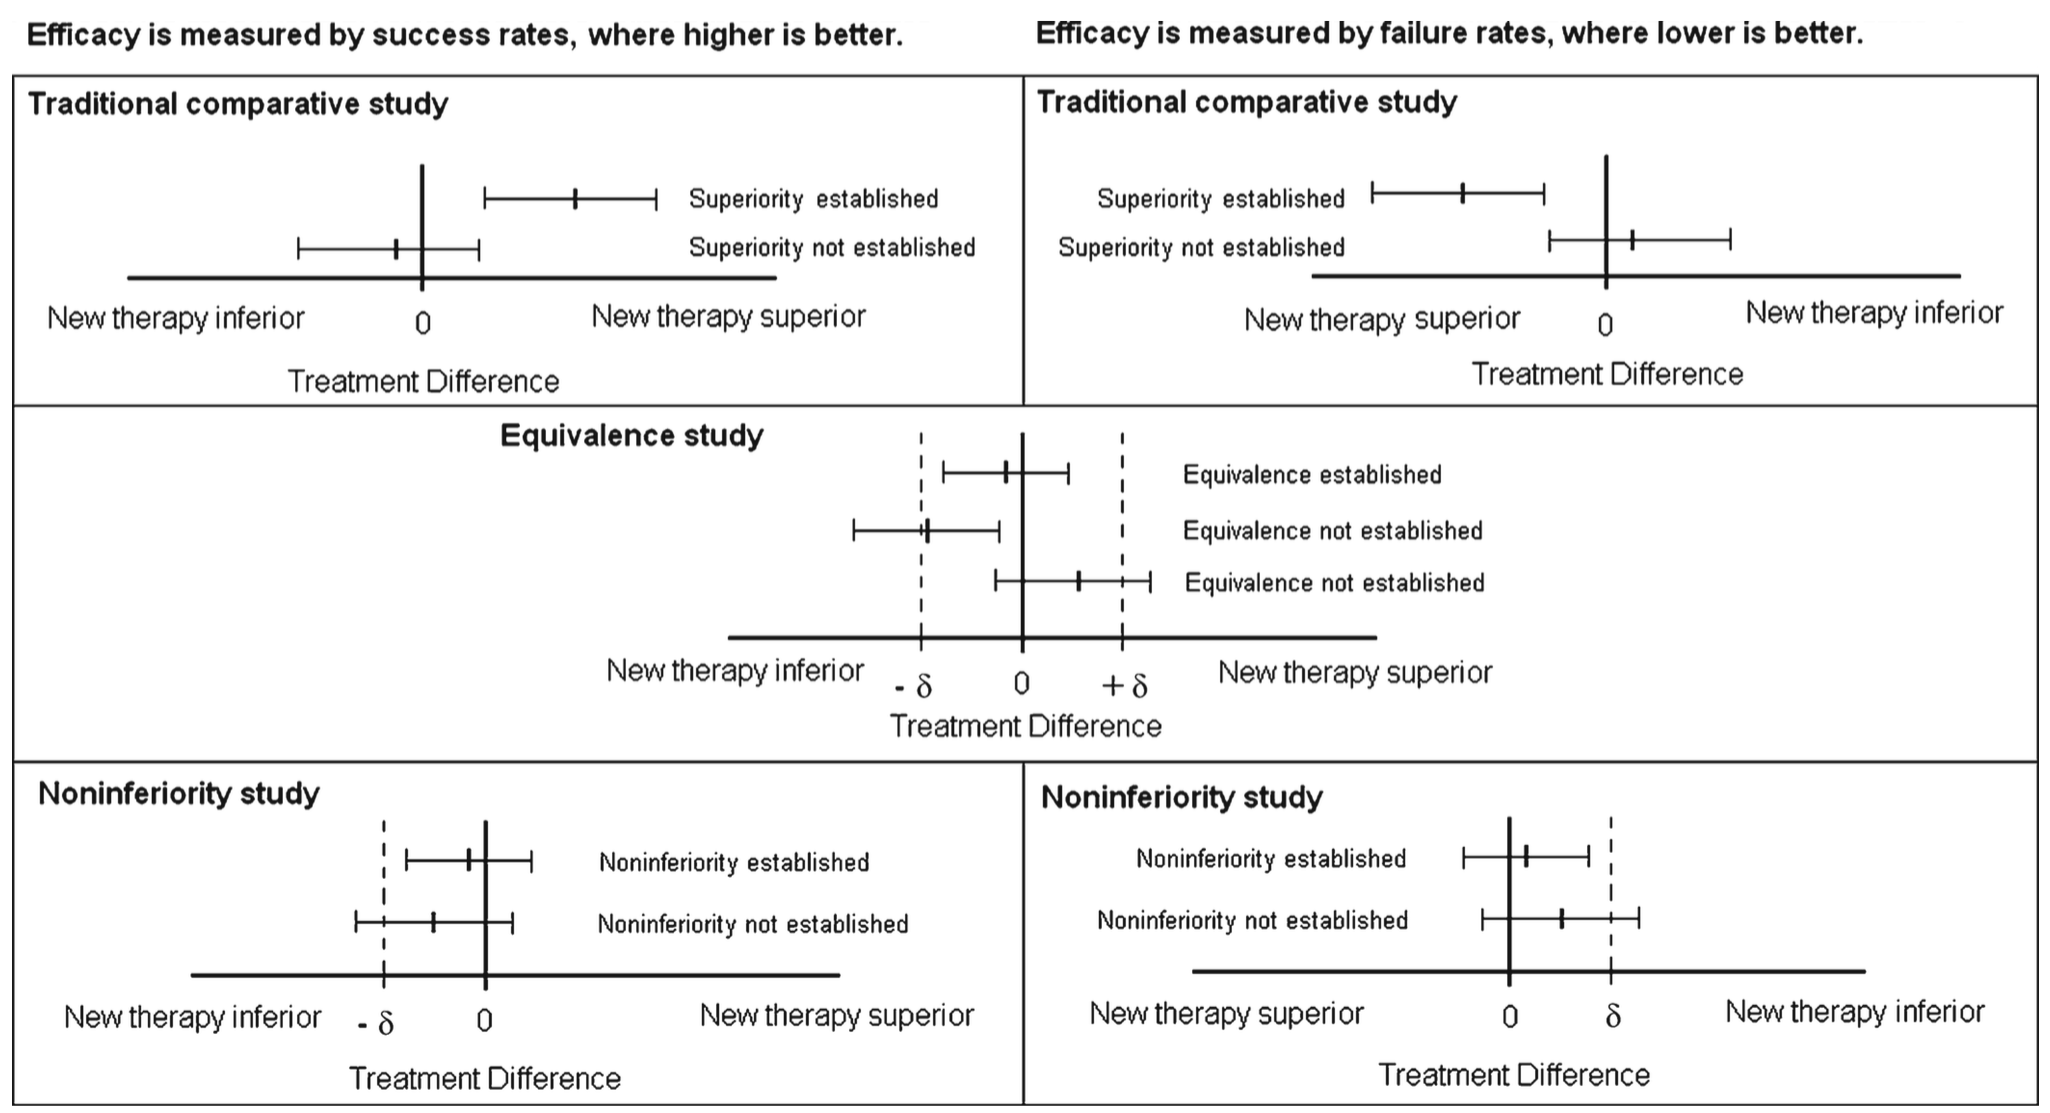
\includegraphics[width=\textwidth]{../img/TOST.png}
\ppagenote{Summary of Equivalence Testing: Walker and Nowacki (2011), J. General Internal Medicine 26(2):192-196.}
\end{frame}


\begin{frame}{Testing Equivalence}{Quick-and-dirty approach}
A simple way of thinking about testing equivalence of two means is to observe confidence intervals instead of p-values:

\begin{exampleblock}{}
\centering ``\textit{Equivalence can be established at the $\alpha$ significance level if a $(1-2\alpha)$-confidence interval for the difference between the two means is contained within a interval $\pm\delta^*$.}''
\end{exampleblock}

The difference between testing for differences and for equivalence can be easily illustrated using this approach:

\centering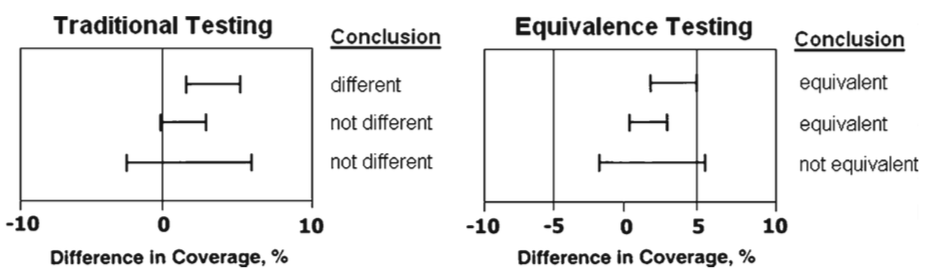
\includegraphics[width=.8\textwidth]{../img/DiffVxEquiv.png}
\ppagenote{Difference vs Equivalence Image: Walker and Nowacki (2011), J. General Internal Medicine 26(2):192-196.}
\end{frame}

\begin{frame}{Equivalence test for a single mean}{Hypotheses}
An equivalence test for a single population mean can be expressed by the hypotheses:
\begin{equation*}
  \begin{cases}
  H_0: \left|\mu-\mu_0\right| = &\Delta\mu \geq\delta^*\\
  H_1: &\Delta\mu <\delta^*
  \end{cases}
\end{equation*}
\medskip

The most usual way of testing these hypotheses is the TOST (\textit{two one-sided tests}) method. As the name suggests, two one-sided significance tests are constructed so that the desired statistical properties can be achieved. Using our standard notation:
\begin{columns}[T]
\column{0.5\textwidth}
\begin{equation*}
\begin{cases}
H_0^1: &\Delta\mu = -\delta^*\\
H_1^1: &\Delta\mu > -\delta^*
\end{cases}
\end{equation*}
\column{0.5\textwidth}
\begin{equation*}
\begin{cases}
H_0^2: &\Delta\mu = \delta^*\\
H_1^2: &\Delta\mu < \delta^*
\end{cases}
\end{equation*}
\end{columns}
\bigskip
If both tests reject their respective $H_0$, then equivalence (within the equivalence margin $\delta^*$) can be declared with significance level $\alpha$.
\end{frame}

\begin{frame}{Interpretation of the Two One Sided Hypothesis}
\centering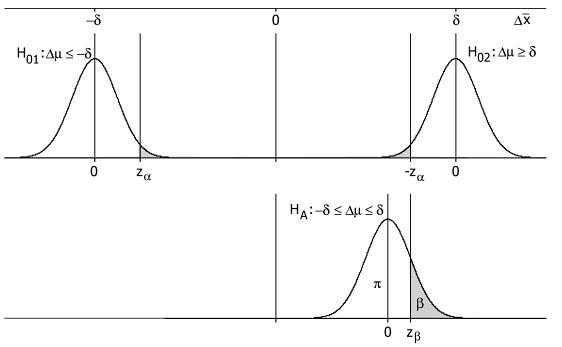
\includegraphics[width=.9\textwidth]{../img/TOST-errors.png}
\ppagenote{TOST errors image: Matthews (2010), Sample Size Calculations, MMB. pg. 46}
\end{frame}


%% Sample sizes
% \begin{frame}{Equivalence of a single mean}{Sample size}
% Sample sizes for testing equivalence of a single mean can be derived using essentially the same considerations used for the usual tests. In the case of a single sample:
% \begin{equation*}
% n\geq\left(\frac{\left(t_{\alpha}+t_{\beta}\right)\hat{\sigma}}{\delta^* - \Delta\mu}\right)^2
% \end{equation*}
% \bigskip
%
% As in the previous cases, iteration is needed to solve for $n$ (since the quantiles of the t distribution depend on $n$). Use $t_x$ = $z_x$ for the first iteration.
% \end{frame}


\begin{frame}{Equivalence Testing by TOST}{Hypotheses for two samples}
Analogously to the single sample test of equivalence, the hypotheses for testing the equivalence of two population means can be described as:
\begin{equation*}
\begin{cases}
H_0: &\mu_1-\mu_2 \geq\delta^*\\
H_1: &\mu_1-\mu_2 <\delta^*
\end{cases}
\end{equation*}
\hrulefill

\begin{columns}[T]
\column{0.5\textwidth}
\begin{equation*}
\begin{cases}
H_0^1: &\mu_1-\mu_2 = -\delta^*\\
H_1^1: &\mu_1-\mu_2 > -\delta^*
\end{cases}
\end{equation*}
\column{0.5\textwidth}
\begin{equation*}
\begin{cases}
H_0^2: &\mu_1-\mu_2 = \delta^*\\
H_1^2: &\mu_1-\mu_2 < \delta^*
\end{cases}
\end{equation*}
\end{columns}
\bigskip

Just as in the previous case, both hypotheses are tested at the desired $\alpha$ value, and the rejection of both $H_0$ indicates evidence of equivalence.
\end{frame}



% \begin{ftst}
% {Equivalence of two means}
% {Sample size}
% Sample size for the $n_1 = n_2 = n$ case can be approximated based on the Zhang formula\footnote[1]{\tiny Zhang (2003), J. Biopharm. Stat. 13(3):529-538.}:
% $$n \geq \left(t_{\alpha;\nu}+t_{(1-c)\beta;\nu}\right)^2\left(\frac{\hat{\sigma}_1^2+\hat{\sigma}_2^2}{\delta^*-\Delta\mu^*}\right)^2$$
%
% \noindent with $\Delta\mu^*<\delta^*$ as the maximum real difference between the two means for which a power of $(1-\beta)$ is desired, and:
% $$c = \frac{1}{2}\exp\left(-7.06\frac{\Delta\mu^*}{\delta^*}\right)$$
%
% The degrees of freedom $\nu$ of the t-quantiles are given by the Welch t-test formula (see Chapter 6).
% \end{ftst}
%
% %=====
%

\subsection{Example}

\begin{frame}{Example -- Laboratory certification}

\begin{columns}[T]
  \column{0.7\textwidth}
  A ballistics laboratory is in the process of being certified for the evaluation of shielding technology, and needs to provide evidence of equivalence of a given callibration procedure with the reference equipment;
  \column{0.3\textwidth}
  
\includegraphics[width=\textwidth]{../img/Shotgun-Ballistic-Shield.png}
  \ppagenote{Gun Shield Image from: \url{http://www.everydaynodaysoff.com/2013/08/05/ballistic-shield-for-operators-only/}}
\end{columns}
\bigskip

The certification authority demands that the mean hole area generated by this procedure in the lab be the same as the one from the reference equipment, and tolerates deviations no greater than $4 mm^2$;
\bigskip

From previous measurements, the standard deviations can be roughly estimated as $\hat{\sigma}_{Lab} = 5 mm^2$ and $\hat{\sigma}_{ref} = 10 mm^2$.
\bigskip

The desired error levels for the comparison are $\alpha=0.01$ and $\beta = 0.1$.
\end{frame}

\begin{frame}[fragile]{Example -- Laboratory certification}
To calculate the required sample size, assume that $\Delta\mu^* = 0.5$. Then:
\begin{verbatim}
> # load functions to calculate sample size for TOST
> source("calcN_tost.R")
>
> # Calculate sample size
> calcN_tost2(alpha = 0.01,
+             beta = 0.1,
+             diff_mu = 0.5,
+             tolmargin = 4,
+             s1 = 5,
+             s2 = 10)
[1] 144.1999
\end{verbatim}
\medskip
We'll need 145 observations from each group to test for equivalence with the desired experimental properties.
\end{frame}

\begin{frame}[fragile]{Certification -- Data Analysis}
After collecting the observations, we proceed to the analysis:
{\tiny
\begin{verbatim}
> data<-read.table("../data files/labdata-example.csv",
+                  header = T, sep = ",")

> # Two one-sided t-tests
> t.test(HoleArea~Place,  data = data,  alternative = "less", mu = 4,
+        conf.level = 0.99)$p.value
[1] 0.00304124
> t.test(HoleArea~Place, data = data, alternative = "greater", mu = -4,
+        conf.level = 0.99)$p.value
[1] 6.586193e-10

> # Get (1-2*alpha) CI
> t.test(HoleArea~Place, data = data,  conf.level = 0.98)$conf.int
[1] -0.5117627  3.6244386
\end{verbatim}}

\hfill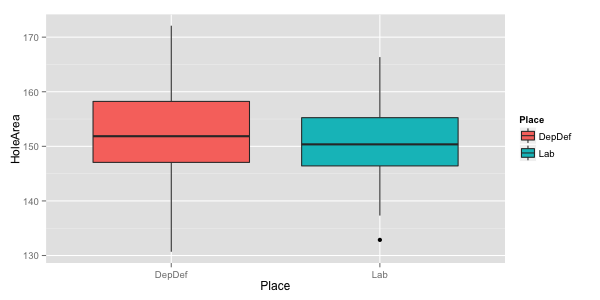
\includegraphics[width=.45\textwidth]{../img/labdata.png}
\end{frame}


\begin{frame}[fragile]{Verification of test assumptions -- Normalty}
\hfill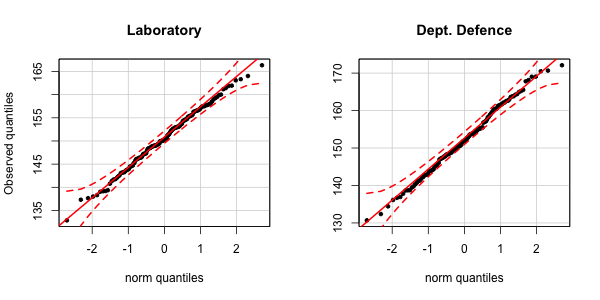
\includegraphics[width=.6\textwidth]{../img/labdata-qqplots.png}
{\smaller
\begin{verbatim}
> par(mfrow=c(1,2))
> qqPlot(subset(data, Place=="Lab")[,2],
+        pch=20,
+        main = "Laboratory",
+        ylab = "Observed quantiles")
> qqPlot(subset(data, Place=="DepDef")[,2],
+        pch=20,
+        main = "Dept. Defence",
+        ylab = " ")
\end{verbatim}}
\end{frame}

\begin{frame}[fragile]{Verification of test assumptions -- Independence}

{\smaller
\begin{verbatim}
> dwtest(HoleArea~Place, data=data)
DW = 1.8116, p-value = 0.04757

> par(mfrow=c(1,2))
> plot(seq_along(subset(data, Place=="Lab")[,2]),
+      subset(data, Place=="Lab")[,2], ...)
> plot(seq_along(subset(data, Place=="DepDef")[,2]),
+      subset(data, Place=="DepDef")[,2], ...)
\end{verbatim}}

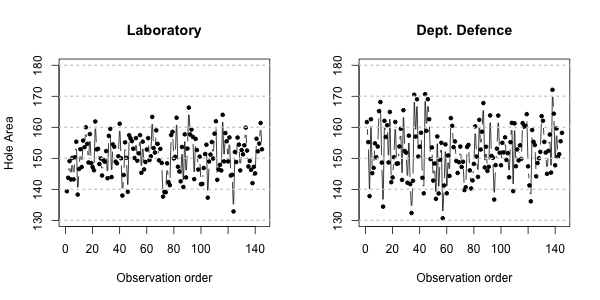
\includegraphics[width=.7\textwidth]{../img/labdata-resplot.png}
\end{frame}
